\begin{tikzpicture}
    \draw[color=lightgray, fill=lightgray] (0.5,0) rectangle (3.5,1);
    
    \draw[color=gray!50!black, fill=gray!50!black] (2.95,0) rectangle (3,1)node[color=gray!50!black,right = 0.1 cm, above]{$\substack{\text{composante }\infty\\ \text{fine de l'ASE}}$};
    \draw[color=blue!50!cyan, fill=blue!50!cyan] (1.45,0) rectangle (1.5,1)node[color=blue!50!cyan,left= 0.5 cm, above]{$\substack{\text{composante }\infty\\ \text{fine de l'ASE}}$};
    \draw[thick,->] (2,0) --++ (0,2) node[above]{signal};
    \draw[thick,->] (0,0) --++ (4,0) node[right]{$\nu$};
\end{tikzpicture}
